\section{Разработка программного средства}
Библиотека Spray, описанная в раздела ~\ref{sec:techs:spray}, имеет очень выразительный внутренний язык описания разбора, обработки и маршрутизации запросов к сервису. Модуль доступа к данным является связующий звеном между модулями приложения и базой данных. Поскольку одной из задач программного средства является предотвращение не авторизированного доступа к данным.
Метод маршрутизации запросов к серверу


Метод классификации образца почерка 
\lstinputlisting[
    style=commonstyle,
    caption=Пример файла конфигурации модуля,
    label=lst:development:classification
]{src/evaluate_single_instance.java}

Пример JSON-документа описывающего образец текста 
\lstinputlisting[
    style=commonstyle,
    caption=Пример JSON-документа описывающего образец текста,
    label=lst:development:json:sample
]{src/sample_item.json}

Пример JSON-документа описывающего пользователя
\lstinputlisting[
    style=commonstyle,
    caption=Пример JSON-документа описывающего пользователя,
    label=lst:development:json:user
]{src/user_item.json}

Маршрутизация запросов к серверу в модуле доступа к данным
\lstinputlisting[
style=commonstyle, 
caption=Маршрутизация запросов к серверу в модуле доступа к данным,
label=lst:development:db_rout
]{src/routing.scala}

\begin{figure}[ht]
    \centering
    \label{fig:develoipment:class_fdp}
    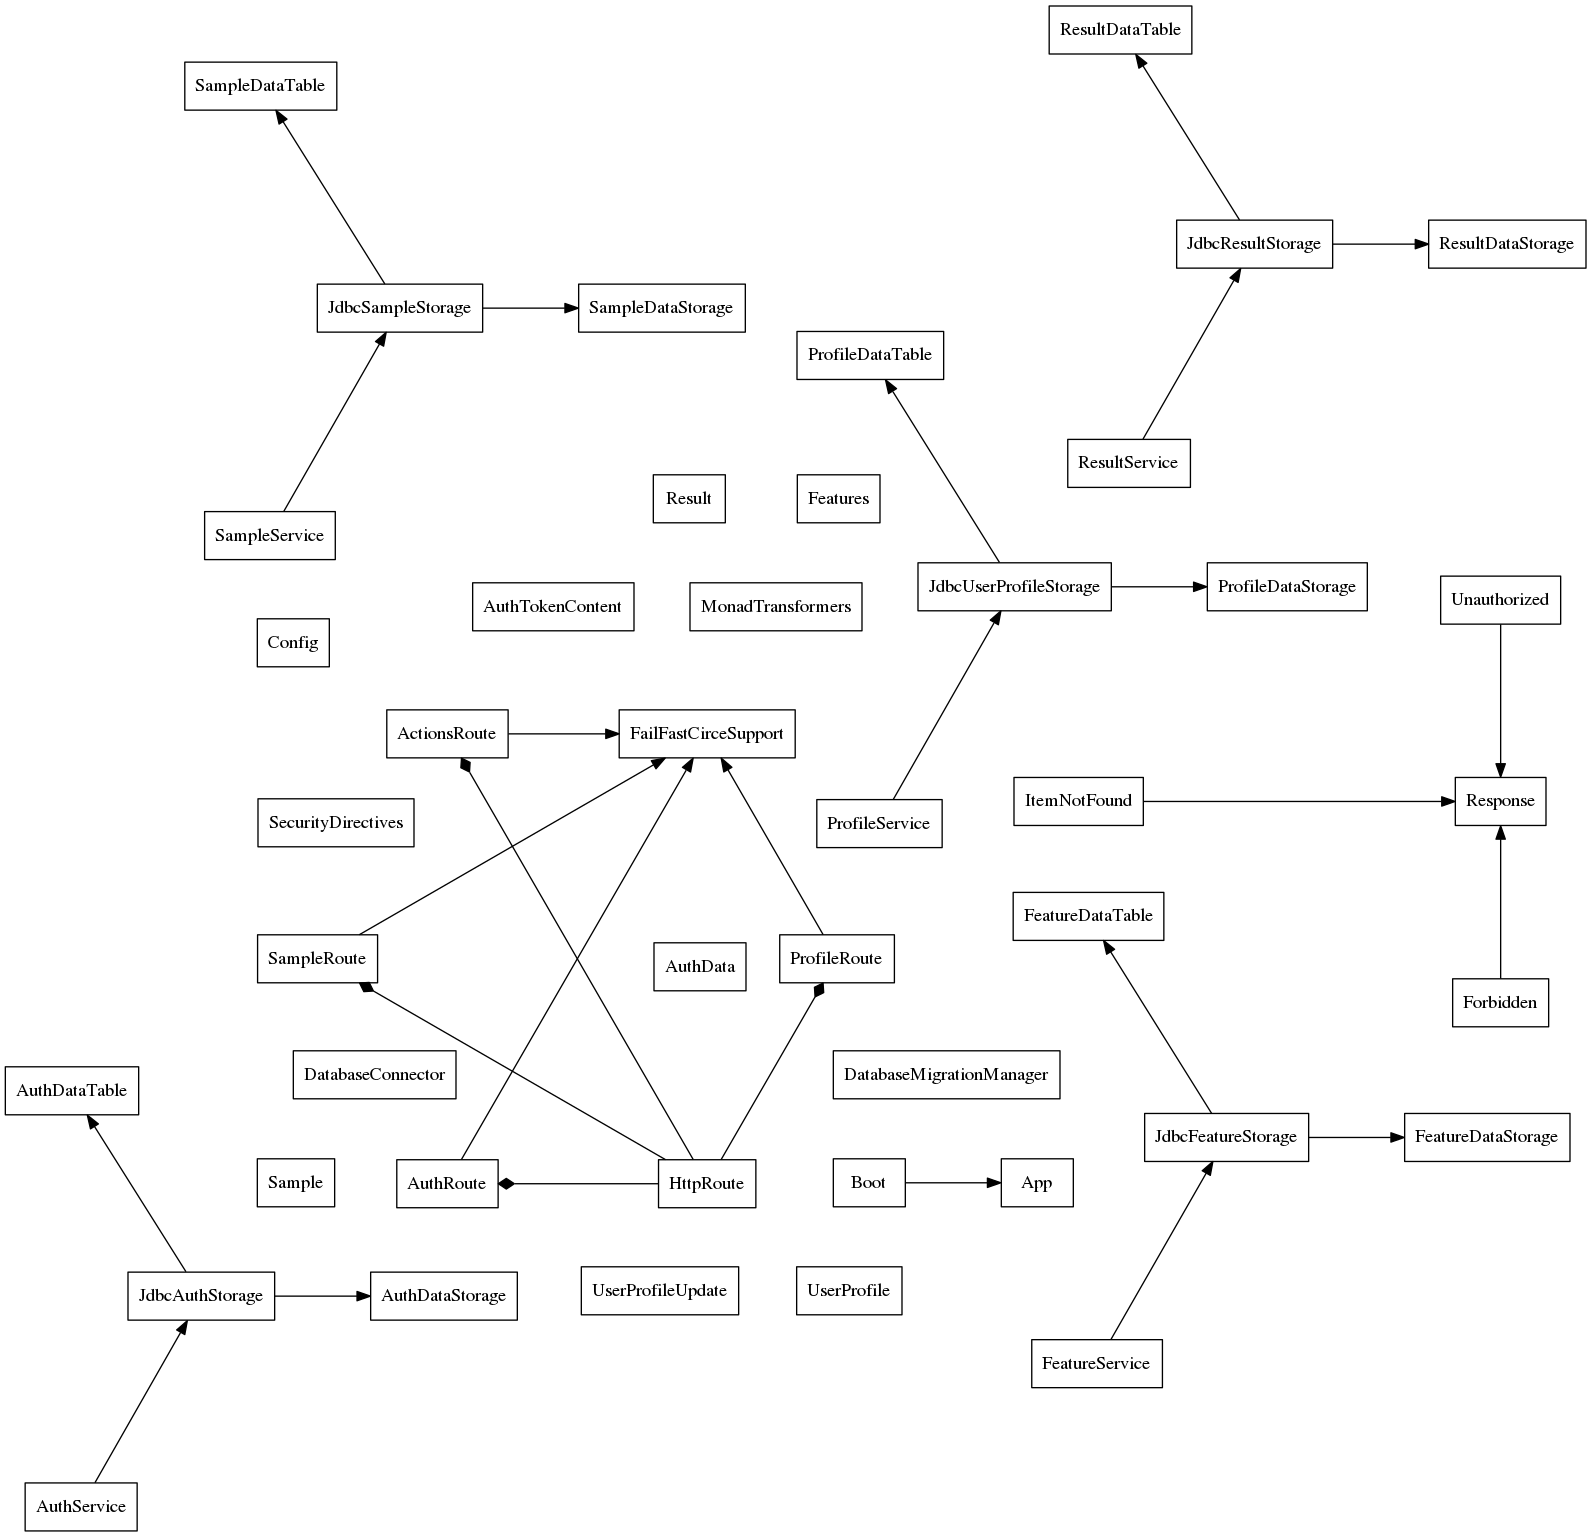
\includegraphics[width=1\textwidth]{figures/classes-fdp.png}
    \caption{Иерархия классов}
\end{figure}

\begin{figure}[ht]
    \centering
    \label{fig:develoipment:svm_flow}
    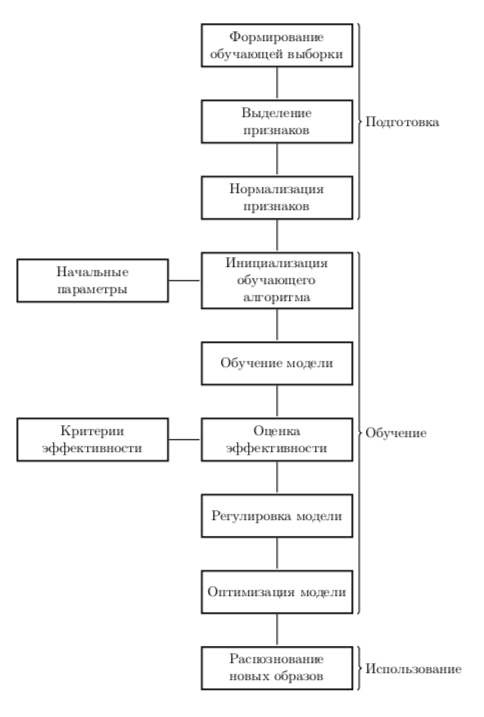
\includegraphics[width=1\textwidth]{figures/SVM_flow.png}
    \caption{Алгоритм обучение}
\end{figure}